\documentclass{aastex62}
\usepackage[utf8]{inputenc}
\usepackage{natbib}
\usepackage{listings}
\usepackage{xspace}
\usepackage{paralist}

% for notes support
% \usepackage{geometry}
% \geometry{right=1.5in}

\newcommand{\package}[1]{\texttt{#1}\xspace}
\newcommand{\code}[1]{\texttt{#1}\xspace}
\newcommand{\github}{\package{GitHub}}
\newcommand{\python}{\package{Python}}

\newcommand{\sunpyproj}{SunPy project\xspace}
\newcommand{\sunpypkg}{\package{sunpy}}
\newcommand{\sunpycode}[1]{\code{#1}}

\newcommand{\astropy}{Astropy\xspace}
\newcommand{\astropypkg}{\package{astropy}}

\newcommand{\numpy}{NumPy\xspace}

\newcommand{\Map}{\sunpycode{Map}}
\newcommand{\Timeseries}{\sunpycode{TimeSeries}}
\newcommand{\Timeseriesmetadata}{\sunpycode{TimeSeriesMetaData}}
\newcommand{\Spectra}{\sunpycode{Spectra}}
\newcommand{\Fido}{\sunpycode{Fido}}
\newcommand{\Lightcurve}{\sunpycode{LightCurve}}
\newcommand{\GenericTimeSeries}{\sunpycode{GenericTimeSeries}}
\newcommand{\GenericMap}{\sunpycode{GenericMap}}

\newcommand{\hpc}{helioprojective Cartesian\xspace}
\newcommand{\hcc}{heliocentric Cartesian\xspace}
\newcommand{\hgs}{heliographic Stonyhurst\xspace}
\newcommand{\hgc}{heliographic Carrington\xspace}
\newcommand{\hpcframe}{\package{HelioprojectiveCartesian}}
\newcommand{\hccframe}{\package{HeliocentricCartesian}}
\newcommand{\hgsframe}{\package{HeliographicStonyhurst}}
\newcommand{\hgcframe}{\package{HeliographicCarrington}}

\shorttitle{Sunpy Project II}
\shortauthors{The SunPy Community}

% Words that should not be hyphenated
\hyphenation{NumFOCUS}

% For commenting - can be deleted before submission
%\usepackage[colorinlistoftodos]{todonotes}
%\newcommand{\inlinecomment}[2]{\todo[inline]{#1: #2}\xspace}
%\newcommand{\comment}[2]{\todo{#1: #2}\xspace}

\begin{document}

\title{The \sunpyproj: Open Source Development and Status of the v1.0 Core Package}
\author[0000-0000-0000-0000]{The SunPy Community}
\noaffiliation

% \author[orcid-id]{name}
% \affiliation{}

% the following author list organization is TBD.

% below add contributing authors (those folks that have actually worked writing the paper) this list should be ordered by contribution like a normal paper. 
% The order is TBD.
\author[0000-0001-6127-795X]{Steven D. Christe}
\affiliation{NASA Goddard Space Flight Center, Greenbelt, MD, USA}

\author[0000-0003-4217-4642]{Stuart Mumford}
\affiliation{DKIST}
\affiliation{aperio software}

\author[0000-0000-0000-0000]{Daniel F.\ Ryan}
\affiliation{NASA Goddard Space Flight Center, Greenbelt, MD, USA}
\affiliation{Catholic University of America, Washington, DC, USA}

\author{Nabil Freij}
\affiliation{aperio software}

\author[0000-0002-5662-9604]{Monica G.\ Bobra}
\affiliation{W.W. Hansen Experimental Physics Laboratory, Stanford University, Stanford, CA 94305, USA}

\author{Jack Ireland}
\affiliation{NASA Goddard Space Flight Center, Greenbelt, MD, USA}

\author{Laura Hayes}
\affiliation{NASA Goddard Space Flight Center, Greenbelt, MD, USA}

\author{Albert Y. Shih}
\affiliation{NASA Goddard Space Flight Center, Greenbelt, MD, USA}

\author{Russel Hewett}
\affiliation{An affiliation}
\author{Kevin Reardon}
\affiliation{An affiliation}

\author{David Perez-Suarez}
\affiliation{An affiliation}

\author{Sabrina Savage}
\affiliation{NASA Marshall Space Flight Center, Huntsville, AL, USA}

\collaboration{(Primary Paper Contributors)}

% Below add contributors to the Sunpy project
% this list is ordered alphabetically
\author{contributor author1}
\affiliation{An affiliation}

\author{contributor author2}
\affiliation{An affiliation}

\author{contributor author3}
\affiliation{An affiliation}

\author{contributor author4}
\affiliation{An affiliation}

\collaboration{(Sunpy Contributors)}

\correspondingauthor{Steven Christe}
\email{steven.christe@nasa.gov}
\begin{abstract}
    The primary goal of the \sunpy Project is to facilitate and promote the use and development of a community-led, free and open-source software for solar physics based on the scientific \python environment. This goal is primarily achieved through the development of the \sunpypkg core package which aims to provide foundational capabilities to the community. The Project also supports a number of  affiliated package which depend on the core package. The aim of this paper is to describe the first official stable release (v1.0) of the core package as well as the project organization and infrastructure. This paper concludes with a discussion of the future of the Project.
\end{abstract}
\date{\today}

\section{Introduction}
\label{sec:intro}

Heliophysics as a discipline is the study of the Sun and its interactions with the solar system.
The Heliophysics community includes many people studying various sub-domains: the Sun, the solar wind, space weather, terrestrial and planetary magnetospheres, the heliosphere, and the Earth's ionosphere, thermosphere, and mesosphere.
Advancing our understanding of the fundamental processes underpinning this complex system requires interdisciplinary research across these scientific sub-disciplines.
At the time of writing, the NASA Heliophysics System Observatory consists of 18 missions with nearly 200 instruments.

Software packages to analyze data from these instruments are generally developed independently by each instrument team.
This creates a diverse and therefore difficult data and software environment to navigate.
Scientists conducting interdisciplinary research from multiple instruments run into problems with incompatible data formats and incompatible analysis routines written with different versions of the base code. Further, it is difficult to reproduce others' scientific results without open data and version-controlled open source software.

A common, version-controlled, open source platform that provides a standard interface to data products and encourages the re-use of common functions can go a long way toward solving this problem.
\sunpy aims to provide this solution for the field of solar physics.

The mission statement of the \sunpyproj is to facilitate and promote the use and development of several community-led, free, and open-source\footnote{\url{https://opensource.org/osd}} data analysis software packages based on the scientific \python\footnote{\url{https://www.python.org/}} environment.
To achieve this goal, the project primarily develops and maintains a core package (\sunpypkg) and supports an ecosystem of affiliated packages (see Section \ref{sec:affil_packages}) that provides additional functionality.

The \sunpyproj was formally founded in March of 2014.
The project selected the \python programming language to leverage the rich ecosystem of packages already available for general data analysis.
These include \package{Numpy} for multi-dimensional array manipulation \citep{numpy}, \package{scipy} for scientific functions \citep{scipy}, \package{Matplotlib} for publication-quality 2D plotting \citep{matplotlib}, and \package{Pandas} for data structures and time series analysis \citep{pandas}.
These core packages form the backbone for hundreds of thousands of additional \python packages.
Of particular relevance to \sunpypkg is the \astropypkg package, which provides core functionality for the analysis of astrophysical data \citep{astropy2018}.

This paper describes the first stable release (v1.0) of the core package.
A previous paper described release v0.5 \citep{Community:2015cy}.

\section{Project Organization \& Enhancement Proposals}

The organization of the \sunpyproj is modeled on the structure of a board-only not-for-profit corporate entity.
It consists of an up-to 10 member self-selected board.
An executive director, elected by the board, forms the core development team, leads the development of \sunpy core package, provides user support, and supports the development of affiliated packages.
As such, the executive director is also the \sunpy lead developer.
A deputy lead developer and release manager, as well as other volunteers from the developer community, support the lead developer.
Board members serve two year terms while the lead developer serves one year terms.

The \sunpyproj is formally defined through \sunpy Enhancement Proposals (SEPs) which are modeled after the Python Enhancement Proposal process\footnote{\url{https://www.python.org/dev/peps/}}.
SEPs are version controlled and publicly available\footnote{\url{https://github.com/sunpy/sunpy-SEP}}.
The first two SEPs (SEP-0001 and SEP-0002) define themselves as well as the \sunpy organization.

SEPs are used to both define the Project as a whole as well as technical requirements for the \sunpypkg core package.
There are generally three types of SEPs.
\begin{itemize}
    \item \textbf{Standard}: Introduces and describes a new feature, or changes to an existing feature, and is meant to function as a high-level technical design document.
    \item \textbf{Process}: Describes a new process, or changes to an existing process, in the \sunpyproj management.
    \item \textbf{Informational}: Provides information and does not introduce any new features, changes, or processes.
\end{itemize}

As of the time of writing, there are a total of 8 SEPs.
Some notable SEPs led to the adoption of physical units throughout the code base (SEP-0003, see Section~\ref{sec:units}), defined the affiliated package program (SEP-0004, see Section~\ref{sec:affil_package}), standardized the use of coordinate and coordinate transformations (SEP-0005, see Section~\ref{sec:coords}), and led to the adoption of a high precision scientific time format (SEP-0008).

\section{Support \& Sustainability}
\label{sec:intro:support}

The \sunpyproj relies largely on unpaid, volunteer efforts from early career scientists.
The project has not received any significant direct financial support for its work facilitating and promoting any open-source and open development software including \sunpy itself.
The \astropy community faces a similar problem \citep{PriceWhelan:2018ji, Muna2016}.

The \sunpyproj does participate in two summer of code programs, which offer students stipends to write code for open-source projects, via the OpenAstronomy umbrella organization.
Since 2013, 16 students contributed to \sunpy through the Google Summer of Code (GSoC)\footnote{\url{https://summerofcode.withgoogle.com/}} program.
Since 2011, 7 students contributed to \sunpy through a similar program funded by the European Space Agency called The ESA Summer of Code in Space\footnote{\url{https://socis.esa.int/}}.
Many \sunpy community members served as mentors for these students\footnote{\url{https://github.com/sunpy/sunpy/wiki/Wall-of-Fame}}.
In 2018, NumFOCUS, a 501(c)(3) public charity which collects and manages tax-deductible contributions for many open-source scientific software packages such as NumPy and AstroPy, gave GSoC student Vishnunarayan K. I. an award for exceptional contributions to the open source scientific software ecosystem for his efforts to update \sunpy with a modern astronomical time system.

The National Academies of Sciences, Engineering, and Medicine's report on Open Source Software Policy Options for NASA Earth and Space Sciences \citep{NAP2018} outlines several solutions to alleviate this problem -- namely that the NASA Science Mission Directorate provide funding for new and existing open source software projects, promote scientists who spend time developing and improving open source software projects, and offer prizes for exemplary contributions to the open source software community.
The National Academies of Sciences, Engineering, and Medicine's report on Reproducibility and Replicability in Science \citep{NAP2019} recommends that funding agencies invest in the research and development of open-source software that support reproducibility.
The \sunpy community supports solutions like these for all relevant funding agencies and furthermore has the ability to accept financial contributions from institutions or individuals through the NumFOCUS organization.

\section{Development Model}

To satisfy the mission statement of the Project, the \sunpy community adopted an open development model.
This development model is widely used within the scientific Python community.
The \sunpy organization and \sunpypkg package are hosted on \github and use Git\footnote{\url{https://git-scm.com/}} as its distributed version control software.
The entire codebase is publicly available and anyone can suggest changes through pull requests.
Since the codebase is licensed under a permissive 2-clause BSD licence\footnote{\url{https://opensource.org/licenses/BSD-2-Clause}}, anyone can redistribute, improve, repackage or use it in a closed environment as long as they credit the \sunpy developers and redistribute the license.
In order to maintain high quality code, every contribution must satisfy the following requirements:
\begin{enumerate}
    \item Code and documentation must follow widely used style guides (PEP 8 and numpydoc).
    \item All new features must be accompanied with documentation.
    This includes code comments, formal documentation, and gallery examples.
    \item Test code must be provided with coverage reports.
    \item Finally, all code must be reviewed and accepted by at least two members of the developer community before it is integrated into the codebase.
\end{enumerate}

\begin{figure}
\begin{tabular}{cc}
  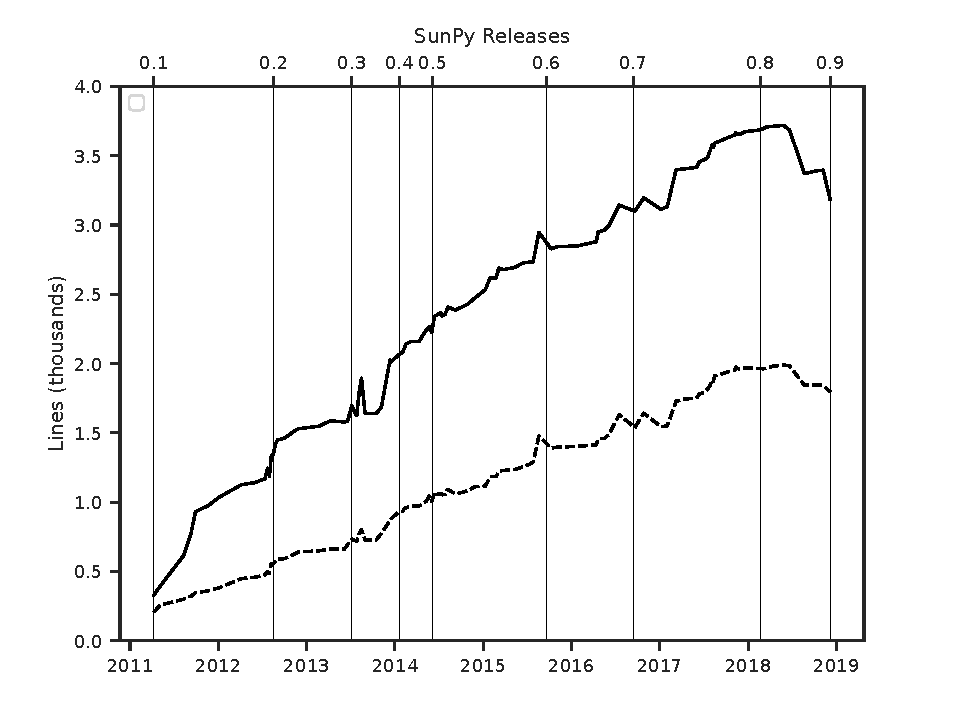
\includegraphics[width=0.5\textwidth]{figures/sunpy_history.pdf} &
  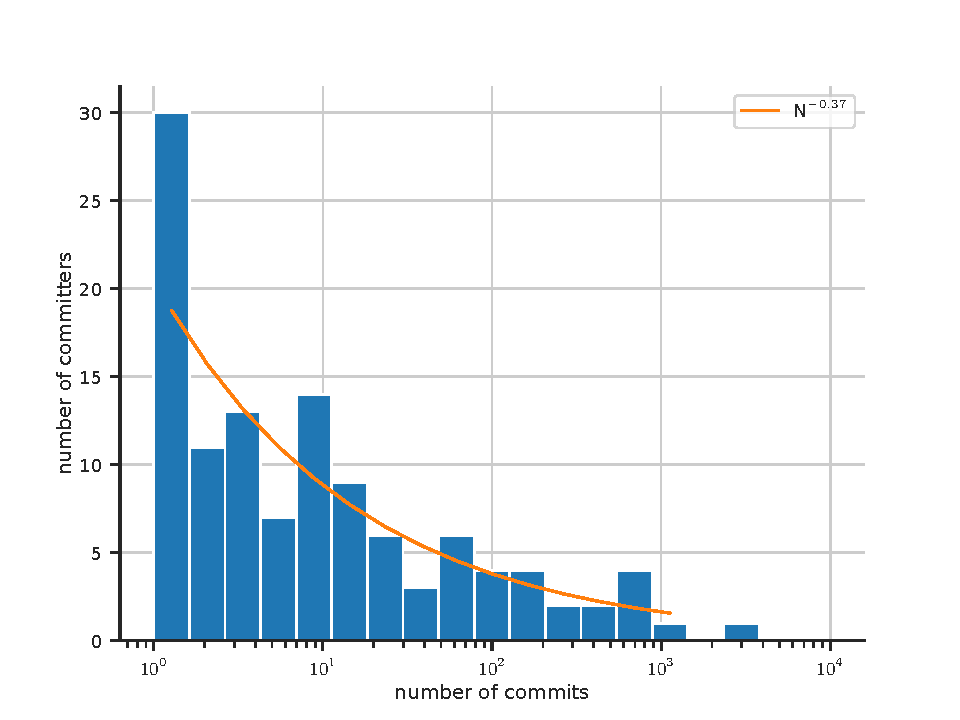
\includegraphics[width=0.5\textwidth]{figures/busfactor_plot.pdf} \\
(a) & (b)  \\
\end{tabular}
\begin{tabular}{c}
  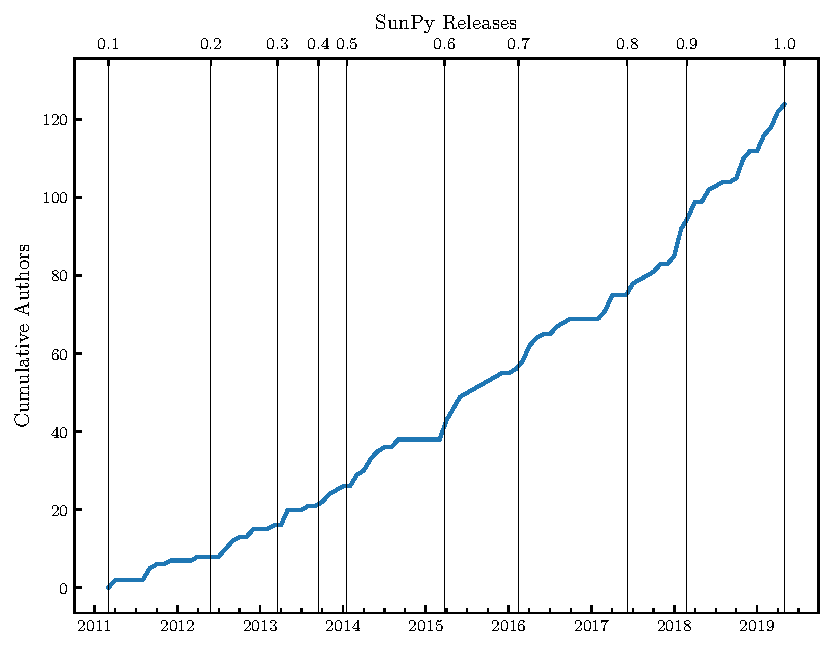
\includegraphics[width=0.5\textwidth]{figures/cumulative_authors.pdf} \\
(c)  \\
\end{tabular}
\caption{
	(a) This figure charts the amount of lines of Python code (dotted black line) and total line count (solid black line) with each major release of \sunpy.
	It details a steady increase of the \sunpypkg codebase with larger additions to our documentation over the last few major versions of \sunpypkg.
	The most striking are the reductions after version 0.9, going into 1.0.
	This was a period that undersaw major phases of code organization, deletion of obsolete features as well as removing Python 2 support.
	(b) This figure showcases the amount of authors to the number of commits they have done.
	It should be noted that the number of commits is not a 100\% useful measure as any one commit could have as many code or line changes as the previous 100 commits.
	However, it does indicate the majority of commits within the package are undertaken by the least amount of people with on average, contributions from an individual is typically less than 10 commits.
	(c) This figure charts the amount of authors (i.e., committers) to the \sunpypkg as a function of time.
	The package has seen a steady rise with time as word of mouth and the community around \sunpy has developed and grown.
	Two periods of time stand out, mid-2015 and early 2018, which saw a large increase in the amount of authors over a shorter period than normal.
}
\label{fig:metafig}
\end{figure}

\section{Project Organization \& Enhancement Proposals}
\label{sec:proj_org}

The organization of the \sunpyproj is modeled on the structure of a board-only not-for-profit corporate entity.
It consists of an up-to 10 member self-selected board.
An executive director, elected by the board, leads the core development team and the development of \sunpypkg core package, provides user support, and supports the development of affiliated packages.
As such, the executive director is also referred to as the lead developer.
A deputy lead developer and release manager, as well as other volunteers from the developer community, support the lead developer.
Board members serve two year terms while the lead developer serves one year terms with no term limits.

The \sunpyproj is formally defined through SunPy Enhancement Proposals (SEPs) which are modeled after the Python Enhancement Proposal process\footnote{\url{https://www.python.org/dev/peps/}}.
All SEPs are version-controlled as well as publicly available\footnote{\url{https://github.com/sunpy/sunpy-SEP}}.
The first two SEPs (SEP-0001 and SEP-0002) define what is an SEP as well as the SunPy organization.

SEPs are used to both define the organization of the project as a whole as well as technical requirements for the \sunpypkg core package and affiliated packages.
There are generally three types of SEPs.
\begin{itemize}
    \item \textbf{Standard}: Introduces and describes a new feature, or changes to an existing feature, and is meant to function as a high-level technical design document.
    \item \textbf{Process}: Describes a new process, or changes to an existing process, in the organization.
    \item \textbf{Informational}: Provides information and does not introduce any new features, changes, or processes.
\end{itemize}

As of the time of writing, there are a total of 8 SEPs.
Some notable SEPs led to the adoption of physical units throughout the code base (SEP-0003, see Section~\ref{sec:units}), defined the affiliated package program (SEP-0004, see Section~\ref{sec:affil_package}), standardized the use of coordinate and coordinate transformations (SEP-0005, see Section~\ref{sec:coords}), and led to the adoption of a high precision scientific time format (SEP-0008).

\section{Support \& Sustainability}
\label{sec:support}

To date, the \sunpyproj relies largely on unpaid, volunteer efforts from early career scientists.
The project has not received any significant direct financial support for its work facilitating and promoting open source and open development software including \sunpypkg itself.
This presents a number of challenges which the \astropy community also faces and are well described in \cite{PriceWhelan:2018ji} and \cite{Muna2016}.

The National Academies of Sciences, Engineering, and Medicine's report on Open Source Software Policy Options for NASA Earth and Space Sciences \citep{NAP2018} outlines several solutions to alleviate these problems -- namely that the NASA Science Mission Directorate provide funding for new and existing open source software projects, promote scientists who spend time developing and improving open source software projects, and offer prizes for exemplary contributions to the open source software community.
The National Academies of Sciences, Engineering, and Medicine's report on Reproducibility and Replicability in Science \citep{NAP2019} recommends that funding agencies invest in the research and development of open source software that support reproducibility.
The SunPy community supports solutions like these for all relevant funding agencies and furthermore has the ability to accept financial contributions from institutions or individuals through the NumFOCUS organization, a 501(c)(3) public charity which collects and manages tax-deductible contributions for many open source scientific software packages such as \numpy and \astropy.

The \sunpyproj does participate in two summer of code programs, which offer students stipends to write code for open source projects, via the OpenAstronomy umbrella organization.
Since 2013, 16 students contributed to \sunpypkg and affiliated packages through the Google Summer of Code (GSoC)\footnote{\url{https://summerofcode.withgoogle.com/}} program.
Since 2011, 7 students contributed through a similar program funded by the European Space Agency called The ESA Summer of Code in Space\footnote{\url{https://socis.esa.int/}}.
Many SunPy community members served as mentors for these students\footnote{\url{https://github.com/sunpy/sunpy/wiki/Wall-of-Fame}}.
In 2018, GSoC student Vishnunarayan K. I. was presented an award by NumFOCUS for exceptional contributions to the open source scientific software ecosystem by updating \sunpypkg with a modern astronomical time system.

\section{Development Model}
\label{sec:development}

To satisfy the mission statement of the Project, the SunPy community adopted an open development model.
This development model is widely used within the scientific Python community.
The\sunpypkg package is hosted on \github and uses Git\footnote{\url{https://git-scm.com/}} as its distributed version control software.
The entire codebase is publicly available and anyone can suggest changes through pull requests.
Since the codebase is licensed under a permissive 2-clause BSD license\footnote{\url{https://opensource.org/licenses/BSD-2-Clause}}, anyone can redistribute, improve, repackage or use it in a closed environment as long as they credit the SunPy developers and redistribute the license.
In order to maintain high quality code, every contribution must satisfy the following requirements:
\begin{enumerate}
    \item Code and documentation must follow widely used style guides (PEP 8 and numpydoc).
    \item All new features must be accompanied with documentation.
    This includes code comments, formal documentation, and gallery examples.
    \item Test code must be provided with coverage reports.
    \item Finally, all code must be reviewed and accepted by at least two members of the developer community before it is integrated into the codebase.
\end{enumerate}
These requirements are imposed on all contributions even those from the SunPy development team.

\begin{figure}
\begin{tabular}{cc}
  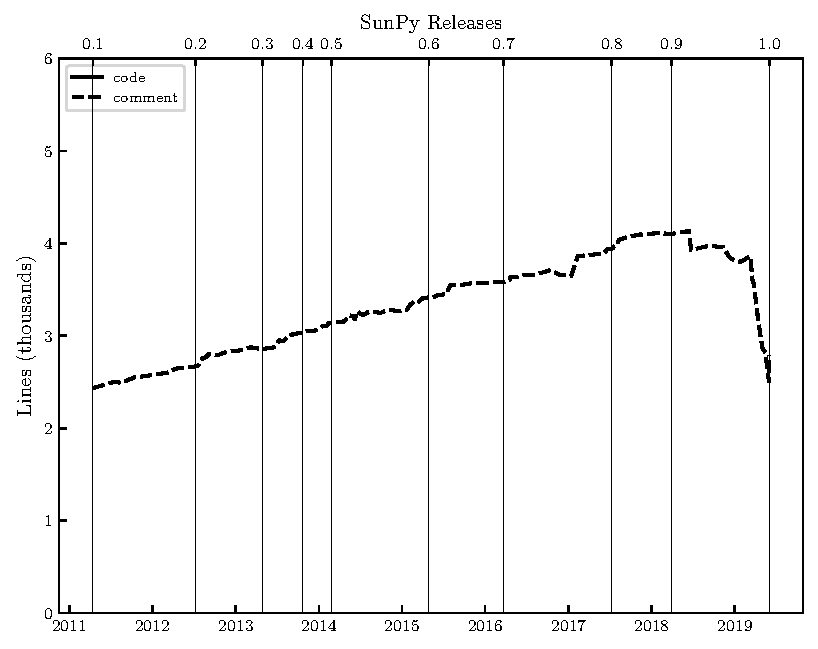
\includegraphics[width=0.5\textwidth]{figures/fig_loc_vs_time.pdf} &
  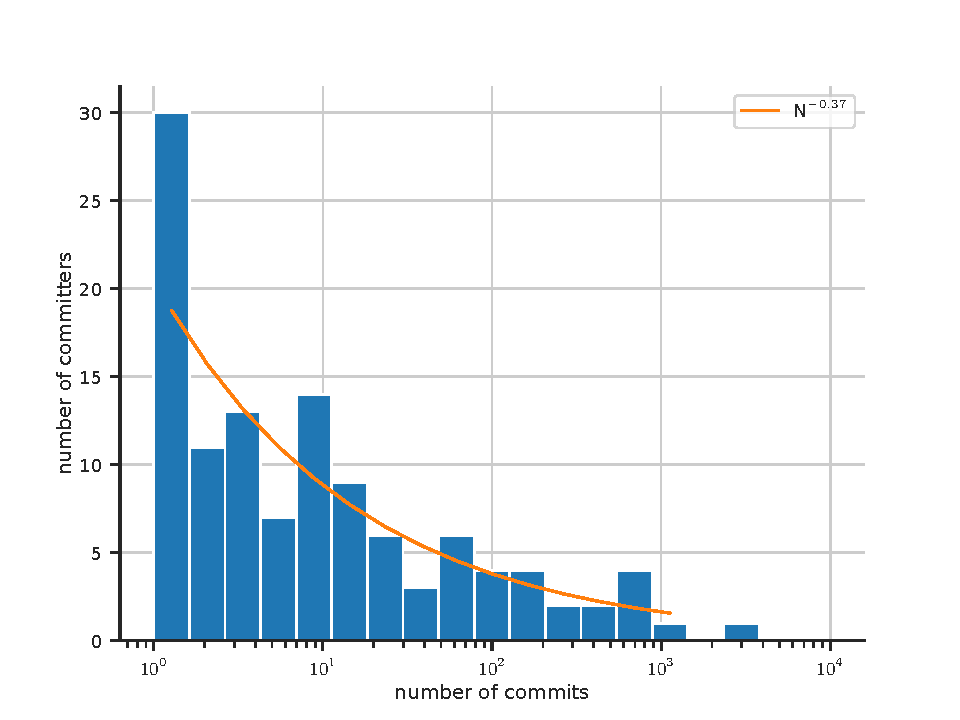
\includegraphics[width=0.5\textwidth]{figures/busfactor_plot.pdf} \\
(a) & (b) \\
\end{tabular}
\begin{tabular}{c}
  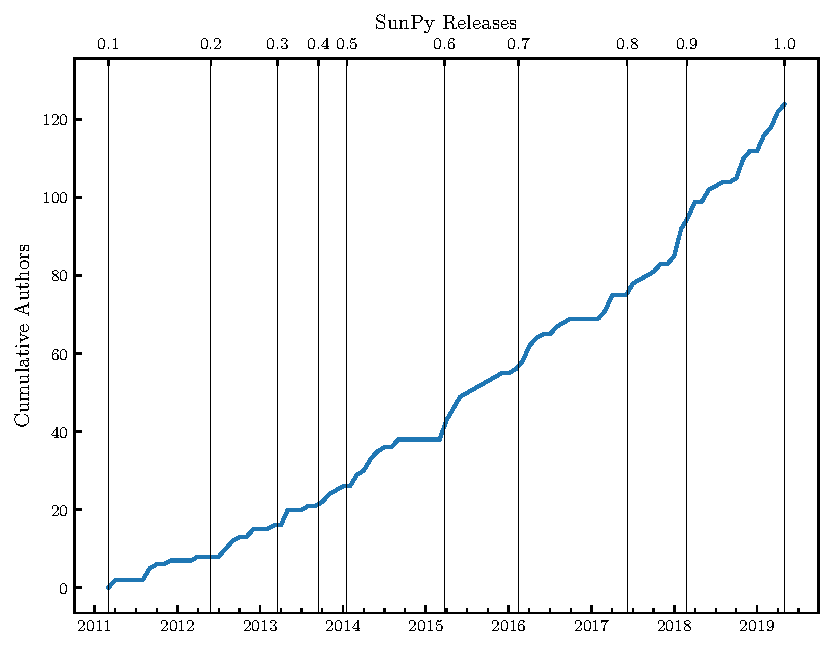
\includegraphics[width=0.5\textwidth]{figures/cumulative_authors.pdf} \\
(c) \\
\end{tabular}
\caption{
	(a) A plot of the the number of lines of code (black line) and documentation line count (dotted black line) as a function of time with major releases.
	It details a steady increase of the \sunpypkg codebase with larger additions to our documentation over the last few major versions of \sunpypkg.
	A striking reduction in the code base occurred after version 0.9.
	During this period a major code organization, deletion of obsolete features as well as removing Python 2 support occurred.
	(b) A plot of the number of authors version number of commits.
	It should be noted that the number of commits is not a 100\% useful measure as any one commit could have as many code or line changes as the previous 100 commits.
	However, it does indicate the majority of commits within the package are undertaken by the least amount of people with on average, contributions from an individual is typically less than 10 commits.
	(c) This figure charts the cumulative number of authors (i.e., committers) to the \sunpypkg as a function of time which shows a steady increase in the number of people that are involved in the development team.
}
\label{fig:metafig}
\end{figure}

\section{Data Types}
\label{sec:data_types}

The \sunpypkg package provides core data types that are designed to provide a standardized interface to data structures across data types (e.g. images and lightcurves) as well as data sources (e.g. from multiple instruments).
The core data types currently provided are \Timeseries and \Map which support 1D temporal data and 2D image data, respectively.
These offer a consistent interface for loading and representing solar data across instruments and missions allowing a simpler work-flow in the analysis of observations.
For example, these core data type classes handle the necessary requirements to read mission specific data and contain the data with a consistent API.
For example, metadata is provided by the \code{.meta} property, and the numeric data is always stored in \code{.data}.
Visualization and basic manipulation routines are also provided.
This section provides an overview of the \Timeseries and \Map classes.

\subsection{\Timeseries}
\label{sec:timeseries}
Time-series data is a fundamental observational data type.
The \Timeseries class provided is designed to handle time-series data through a robust and consistent interface.
\Timeseries supports data from a wide range of instruments.
The inherent structure of the \Timeseries class consists of times and measurements, while the underlying structure used to store the data is a Pandas dataframe.

%The base class of \Timeseries is the \GenericTimeSeries class.
A number of instruments are supported through subclassing which have instrument-specific methods for reading source files.
Custom \Timeseries can also be made from input data in the form of a Pandas dataframe, an Astropy Table or a \numpy array.

\Timeseries currently supports data sources from the following instruments:
Geostationary Operational Environmental Satellite (\textit{GOES}) X-ray Sensor (XRS),
\textit{SDO} EUV Variability Experiment (EVE) \citep{woods2010extreme},
\textit{PROBA2} Large Yield Radiometer (LYRA) \citep{dominique2013lyra},
\textit{Fermi} Gamma-ray Burst (GBM) monitor \citep{meegan2009fermi}
the Nobeyama Radioheliograph (\textit{NoRH}) \citep{nakajima1994nobeyama}
and \textit{RHESSI} \citep{lin2003reuven}.

The \Timeseries\ class also supports the National Oceanic and Atmospheric (NOAA) Space Weather Prediction Center (SWPC) solar cycle monthly indices and predicted progression.
These data sources are supported through a \Timeseries\ instrument source file for each listed above.
With this structure additional instruments and data sources can easily be added.

\Timeseries holds meta data, stored in the \Timeseriesmetadata object.
This functionality is designed to allow the user to create a single \Timeseries by combining multiple \Timeseries together into one, preserving the metadata relevant to each cell, column or row, concatenated into an organized fashion.

\Timeseries also supports manipulation functionality for working with time-series data including adding new columns of data to a \Timeseries, truncating a \Timeseries over a specified time range, resampling, and creating other data products from an existing \Timeseries, such as into a Pandas dataframe or an Astropy table.
The \Timeseries object, similar to \Map (Section \ref{sec:map}), has it's own visualization plotting methods allowing for easy inspection of the data.

\subsection{\Map}
\label{sec:map}

The \Map class provides the functionality to analyze 2D data associated with a coordinate system and relevant metadata.
%A \Map object is created using the \Map factory which will produce a \GenericMap object or a subclass of \GenericMap which deals with instrument specific data.
%The main use of \Map is to store and manipulate images of the Sun and heliosphere.
%A number of instruments are explicitly supported, supported through subclassing within the subclass source files for each instrument source.
Similar to \Timeseries, subclassing provides a compatibility layer which converts the specific meta data and other source-specific parameters to the base class \GenericMap\ interface.
The source files also include properties such as source-specific color tables and appropriate image scaling for each instrument.

\Map currently supports data sources from the following instruments:
\textit{SDO} - Atmospheric Imaging Assembly (AIA) \citep{lemen2011atmospheric} and the Helioseismic and Magnetic Imager (HMI) \citep{scherrer2012helioseismic},
\textit{SOHO} - Large Angle Spectroscopic COronagraph (LASCO) \citep{brueckner1995large}, Extreme ultraviolet Imaging Telescope (EIT) \citep{delaboudiniere1995eit}, and Michelson Doppler Imager (MDI) \citep{scherrer1995solar},
\textit{STEREO} - Extreme Ultraviolet Imager (EUVI), COronagraph 1 and 2 (COR1/2) for both \textit{STEREO} A and B \citep{howard2008sun},
\textit{Hinode} - X-Ray Telescope (XRT) \citep{golub2008x},
\textit{IRIS} Slit Jaw Imager (SJI) \citep{DePontieu2014},
\textit{COronal Solar Magnetism Observatory (COSMO)} - K-coronagraph (K-Cor) all polarized brightness,
\textit{PROBA2} - Sun Watcher using Active Pixel System detector and Image Processing (SWAP) \citep{seaton2013swap},
\textit{RHESSI} \citep{lin2002reuven},
\textit{TRACE}
and \textit{Yohkoh} Soft X-ray Telescope (SXT) \citep{tsuneta1991soft}.
Helioviewer JPEG2000 image files of the above data sources are also supported by the \Map\ class.

A \Map\ can be created either from data files from which the \Map\ factory will automatically detect the type of file, associated instrument and search the appropriate FITS keywords to infer the coordinate system.
A custom \GenericMap can also be created by providing the \Map\ object with data and basic meta information.

Two additional classes based on \Map\ are also provided in \sunpypkg.
The \code{MapSequence} class stores a time-ordered sequence of \Map classes.
The data in each \Map need not have the same size (number of pixels in each direction) or view the same area of sky (field-of-view).
The \code{CompositeMap} class permits the simple overlay and plot of multiple \Map images; such functionality is useful in displaying data from instruments with overlapping fields of view.

\section{Solar Coordinates}
\label{sec:coords}

The \package{sunpy.coordinates} subpackage provides support for representing and transforming solar-centric coordinates. 
These coordinates may represent events (e.g. flares), feature on or above the Sun (e.g. magnetic loops), or  the position of structures traveling throughout the heliosphere such as coronal mass ejections.
The package currently supports many of the most widely used Sun-centered coordinate frames including Helioprojective Cartesian (HPC), Heliographic Carrington (HGC), Heliographic Stonyhurst (HGS),  as well as Heliocentric Aries Ecliptic (HAE), Heliocentric Cartesian (HCC) and Heliocentric Earth Equatorial (HEEQ). 
For more information about these coordinates frames \citep[see][]{2006A&A...449..791T}.
The functionality provided in this package is built on top of and integrates with the \package{astropy.coordinates} framework \citep[see Section 3.3 of][]{astropy2018}.

An important feature of some of these solar coordinate frames is that they are observer-dependent, meaning that they are not fully defined without also specifying the location of the observer.
The HPC frame, in particular, which is the most widely used coordinate frame for images of the Sun, places the origin of the frame at the observed center of the solar disk.
This means that these observer-dependent frames have axes that change orientation depending on the location of the observer, and thus the observer location is necessary to fully define the frame.
In order to accommodate this, all observer-dependent solar coordinates add an observer attribute with the observer coordinate.
Since many observations of the Sun take place from or near the Earth, it is frequently an adequate approximation to use the Earth's location as the observer.

The observer-independent coordinate frames (HAE, HEEQ, HGC, and HGS) are useful for specifying the locations of features on the Sun or objects (e.g., spacecraft) in interplanetary space.
The commonly-used HGS frame is of particular note because it transforms in a straightforward manner to and from the Heliocentric Celestial Reference System (HCRS).
This transformation consists of the combination of two rotation angles: the time-independent angle between the Sun's rotation axis and the HCRS celestial pole \citep[see][]{2007CeMDA..98..155S} and the time-dependent angle of the central meridian (as seen from Earth) relative to the vernal equinox.
This transformation provides the link from the frames defined in \package{sunpy.coordinates} with those defined in \package{astropy.coordinates}, allowing any solar frame to be transformed to and from celestial coordinate frames (\autoref{fig:transform_graph}).
%In fact, HAE is actually implemented in \package{astropy.coordinates}, but the shared framework means that it can be used seamlessly in \sunpypkg.
The functionality provided by  \package{sunpy.coordinates} subpackage has been extensively tested and agrees with published values in the \textit{Astronomical Almanac} to a precision of hundredth of an arcsecond for apparent right ascension.

\begin{figure}
    \centering
    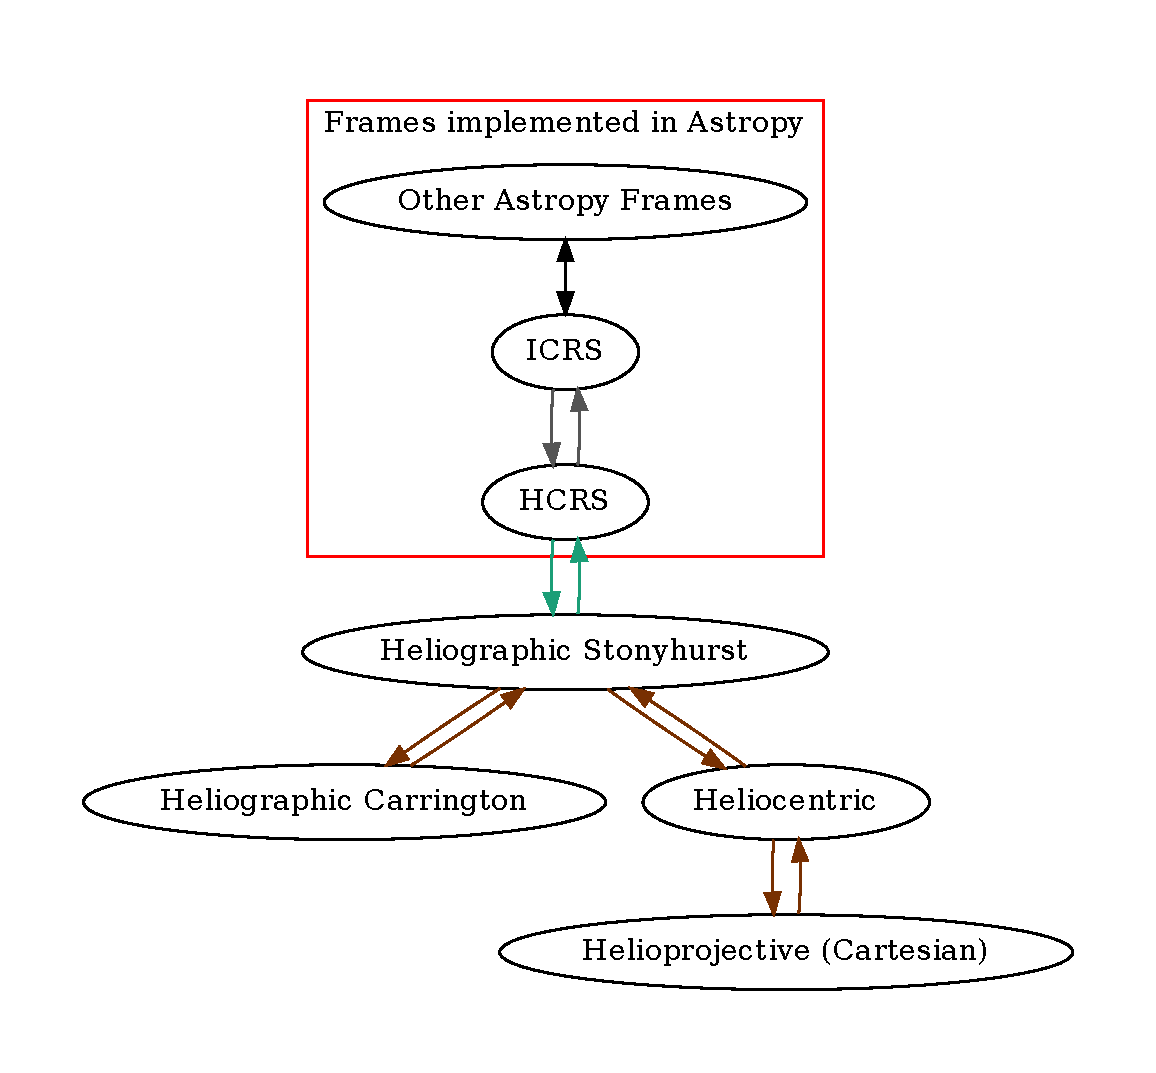
\includegraphics[width=0.75\textwidth]{figures/sunpy_frames.pdf}
    \caption{Graph of the coordinate frames accessible through \package{sunpy.coordinates}, and how they transform between each other.
    The frames within the blue box are implemented in \package{astropy.coordinates}, but in the shared framework, any frame can be transformed to any other frame in this graph.}
    \label{fig:transform_graph}
\end{figure}

A few example applications of the functionality provided by \package{sunpy.coordinates} are shown in \autoref{fig:coordinates_examples}. 
The first panel shows magnetic field line extrapolations projected onto an SDO/AIA 171\AA{} image of an active region.
The center and rightmost panels of \autoref{fig:coordinates_examples} make use of functions in \package{sunpy.coordinates} to obtain the apparent (light-travel time-corrected) location of solar-system bodies and overlay them on images of the Sun in solar coordinate frames .
Support is  provided for querying ephemeris information from a few different sources including the active ephemeris in \package{astropy.coordinates}, JPL ephemeris, and JPL HORIZONS\footnote{\url{https://ssd.jpl.nasa.gov/?horizon}} which also provides ephemeris information of spacecraft such as SDO and SOHO.

\begin{figure}
    \gridline{\fig{figures/fig_fieldlines_aia.pdf}{0.3\textwidth}{(a)}
              \fig{figures/fig_venus_transit.pdf}{0.3\textwidth}{(b)}
              \fig{figures/fig_coronagraph_starfield.pdf}{0.3\textwidth}{(c)}
              }
    \caption{Several example use cases of the coordinate machinery provided by the \package{sunpy.coordinates} subpackage.
    (a) Field lines traced from a potential field extrapolation overlaid on an SDO/AIA 171 \AA{} AIA observation of an active region from 2019 March 10 00:00:04 UTC.
    The field extrapolation was computed with \package{pfsspy} \citep{david_stansby_2019_3237053}.
    (b) The Venus transit as viewed by SDO/AIA in 1600 \AA. The predicted position of Venus is overplotted in the helioprojective coordinate frame of the AIA image.
    (c) A coronagraph image of the solar corona as observed by STEREO-A COR-2. The predicted positions of stars from the Gaia DR2 catalog as well as Mars are overplotted in the helioprojective coordinate frame of the image.}
    \label{fig:coordinates_examples}
\end{figure}

\subsection{Differential Rotation}
\label{sec:differential_rotation}

%1-2 sentences intro; 1-2 sentences describing what is new; 1 sentence that acknowledges the figure.
% Can delete the first two sentences if the background info feels unnecessary

When analyzing the dynamics of features on the solar disk, it is important to account for variations due to the apparent rotation of the Sun.
There are two important effects, the apparent rotation of the Sun as seen from platforms that are orbiting around the Sun such as the Earth and solar differential rotation or the latitudinally-varying rotation rate due to the non-rigidity of the solar interior.
The \package{sunpy.physics.differential\_rotation} subpackage provides tools for correctly accounting for both of these effects on solar coordinates. 
\autoref{fig:diff_rot} shows an example of this functionality applied to a SDO/AIA 1600 \AA{} image which features two prominent active regions. The bottom panel shows the predicted image including differential rotation and the apparent solar rotation due to the observers orbit. This predicted image can be compared to an actual later image by SDO/AIA 1600 \AA{}.

\begin{figure}
    \center
    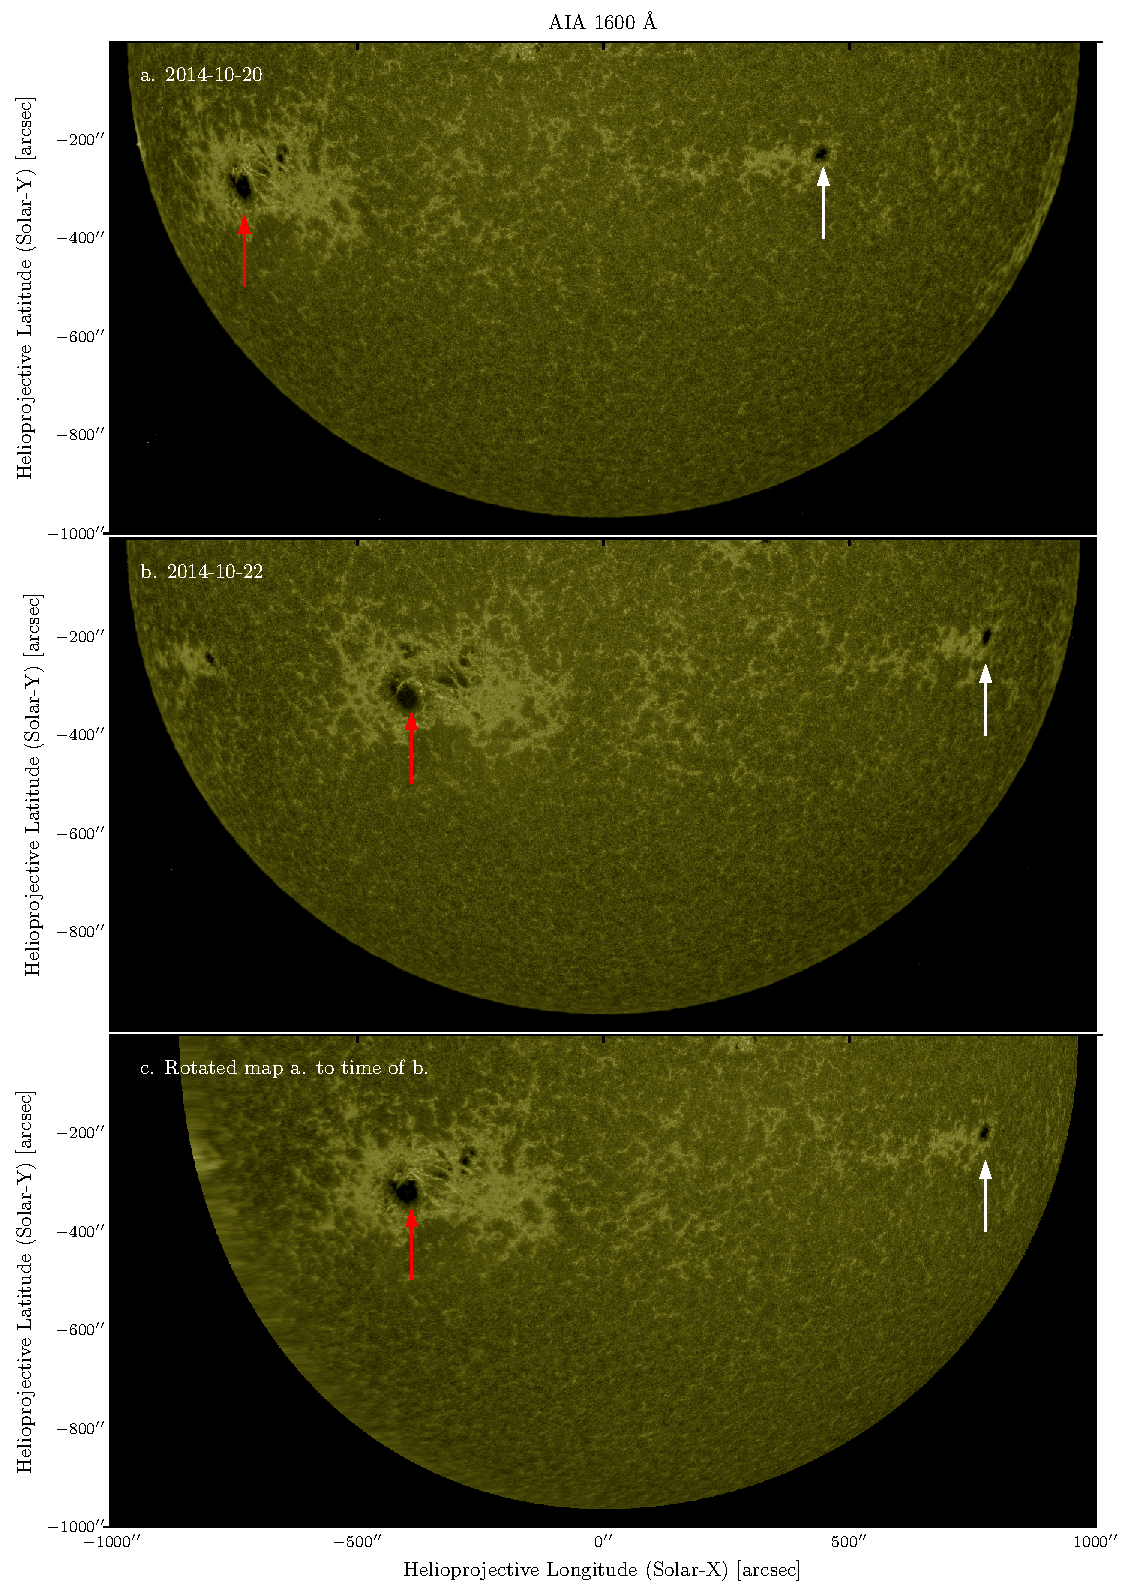
\includegraphics[width = 0.8\textwidth]{figures/fig_diff_rot_1600.pdf}
    \caption{Example of the functionality of \sunpypkg to apply solar differential rotation to a Map.
    Panels (a) and (b) show the Sun as observed in AIA 1600~\AA\ on two different days, 2014-02-20 and 2014-02-22.
    A large sunspot group is highlighted by the red arrow, and a smaller sunspot by the white arrow.
    Panel (c) shows the map of (a) that has been rotated differentially using \sunpypkg to the time of map (b).}
    \label{fig:diff_rot}
\end{figure}

\section{Data search and retrieval}
\label{sec:fido}

One of the most important tasks that must occur before any analysis can take place is to search for and retrieve data.
A particular science goal may require data from multiple data providers, each of which may have different methods of search and retrieval.
This heterogeneity increases the effort required by scientists to get the data they need.
In order to address this issue \sunpypkg provides a single and powerful data search and retrieval interface called \Fido. 

\Fido provides a unified interface that simplifies and homogenizes search and retrieval by allowing data to be queried and downloaded from multiple solar sources simultaneously irrespective of the underlying client.
Currently \Fido supports the Virtual Solar Observatory (VSO), the Joint Science Operations Center (JSOC) (see Section \ref{sec:drms}) and a number of individual data providers that make their data available via web-accessible resources such as HTTP websites (RHESSI, SDO-EVE, NOAA GOES soft X-ray flux, PROBA2-LYRA and NOAA sunspot number prediction) and FTP sites (NOAA sunspot number, Nobeyama Radioheliograph).

A \Fido search can include multiple instruments, and can query all available data providers with a single query.
Search queries make use of search attributes (e.g. instrument, time range, wavelength) which can be joined using Boolean operators enabling complex search queries to be constructed easily.
The result of a query can be inspected and edited before retrieval.

The result of the \Fido search query is downloaded via asynchronous download streams significantly improving download speeds.
\Fido also recognizes failed data downloads and allows for re-requesting files which were not retrieved.

In addition to data download, access to event catalogues are also an important aspect of solar physics research. 
The primary solar event catalog is the Heliophysics Event Knowledgebase (HEK) which provides a searchable database of manually and automatically detected solar features and events such as sunspots, solar flares, coronal mass ejections, etc. \sunpypkg provides a HEK search client which is highly flexible, allowing multiple event types and their properties to be queried simultaneously.
For example, it is possible to search for SPoCA (\cite{2014AA...561A..29V}) active regions above a user-specified size within a given time-range.

Finally, \sunpypkg has a Helioviewer\footnote{\url{https://helioviewer.org/}} client which permits the user to query the Helioviewer JPEG2000 image archive, download image data, and easily construct images of solar data from multiple sources available at the Helioviewer archive.
This will eventually  be moved out of \sunpypkg to an affiliated package in order to expands the scope of the client.

\section{Units and Time Scales}
\label{sec:units}

Calculations using physical quantities have traditionally been performed in software using raw numbers in the interest of simplicity and speed.
The units associated with those numbers would typically be noted separately in comments or in documentation, and that separation between a number and its units can lead to errors or even disaster.
As an extreme example, the Mars Climate orbiter mission in 1988 failed due to a unit discrepancy \citep{mco_mishap_report}.
The spacecraft trajectory was reported in English units instead of metric units, which led to the Mars Climate Orbiter entering the Martian atmosphere well below its intended altitude leading to mission failure.
This mishap could have been avoided by ensuring that physical quantities are fully described in software.

A more modern approach which describes a solution to this problem is provided by \citet{Damevski2009}.
\sunpypkg implements this concept throughout its code base using  functionality provided by \package{astropy.units}.
This subpackage provides support for physical quantities through a class, which consists of a number and its associated unit(s).
Furthermore, these quantities can be combined in expressions with unit conversions and cancellations automatically taken into account.
Tests have shown that the performance overhead to using this functionality is typically minimal.

SEP-0003 formally mandate that all user-facing functionality provided by \sunpypkg make use of this functionality unless inappropriate.
All functions have their input constrained to the appropriate type of unit (e.g. length, mass) and provide an error if the input is not correct.
Input can then be provided with any appropriate units (e.g. mm, km, inches) and conversions occur automatically without user intervention.
The \package{sunpy.sun.constants} subpackage contains many standard constants relevant to solar physics with additional information such as uncertainty and reference.

Time is another fundamental quantity that must be appropriately specified for scientific uses.
Similar motivations led to the adoption of SEP-0008 which mandates the use of a modern scientific time format throughout the \sunpypkg code base.
This functionality is provided by the \package{astropy.time} which provides support for many different time scales, including Coordinated Universal Time (UTC), Terrestrial Time (TT), or International Atomic Time (TAI).
In the same manner as pairing numbers with their units, a time class pairs a time representation with its time scale, and allows for conversions to other time scales.
Thus, functions that require precise times (e.g., for ephemeris calculations) can ensure that there is no confusion about the input.

\section{Affiliated Packages}
\label{sec:affil_package}

In order to foster collaboration, coordination, and code re-use, the \sunpyproj supports the concept of affiliated packages.
These are \python packages that build upon the functionality of the \sunpypkg package or provides general functionality useful to solar physics.
Affiliated packages can also be used to develop and mature subpackage functionality outside of the constraints of \sunpypkg.
The following requirements must be met by potential affiliated packages.
\begin{itemize}
    \item the package must make use of all appropriate features in \sunpypkg,
    \item documentation must be provided that explains the function and use of the package, and should be of comparable quality to \sunpypkg,
    \item a test suite must be provided to verify the correct operation of the package.
\end{itemize}
Developers can formally apply to become an affiliated package to the lead developer and final approval is required by the SunPy board.
Packages are re-reviewed on a yearly basis to ensure that they continue to meet the standards.
All affiliated packages are listed on \url{sunpy.org}, are provided support by the SunPy developer community, and advertised at conferences and workshops.
Sponsored affiliated package are a special class of affiliated package whose maintenance and development is the responsibility of the \sunpyproj.
In order to normalize and as part of the support structure the \sunpyproj provides a package template, \code{sunpy/package-template}\footnote{\url{https://github.com/sunpy/package-template}}, which simplifies packaging, testing, and documentation builds for developers.

The following sections provides short descriptions of the existing affiliated packages.

\subsection{drms}
\label{sec:drms}

The \package{drms} package provides functionality to access data hosted by the Joint Science Operations Center (JSOC).
Operated by Stanford, it is the primary data center for the Solar Dynamics Observatory’s (SDO) Helioseismic and Magnetic Imager (HMI) and Atmospheric Imaging Assembly (AIA) instruments, the Solar and Heliospheric Observatory's (SoHO) Michelson Doppler Imager (MDI) instrument, the NASA Interface Region Imaging Spectrograph (IRIS) Explorer.
DRMS stands for Data Record Management System, a pSQL database that contains metadata, as well as pointers to image data, for every image contained in the archive.
The \package{drms} package provides access to query the rich image metadata in the JSOC DRMS. It can also be used to submit tailored data export requests (e.g. movies and images in various formats) and download data files.
The package is built on the HTTP/JSON interface provided by JSOC.

\subsection{ndcube}
\label{sec:ndcube}

The \package{ndcube} package provides functionality for manipulating N-dimensional coordinate-aware data.
It supports any combination of axis-types for example images (2 spatial axis), images over time (2 spatial and 1 time axis), spectrograms (wavelength and time), as well as more complex data sets such as from slit spectragraphs (wavelength, time, and spatial).
It provides \sunpycode{NDCube} class, a subclass of \astropy's \sunpycode{NDData} data container which hold together the data array uncertainties, and (potentially) a data mask.
\sunpycode{NDCube} adds support for handling world coordinate transformations through the World Coordinate System (WCS) architecture commonly used in solar physics \citep{2002A&A...395.1061G}.
This package provides powerful and intuitive tools for slicing datasets with a single command using either array indices or world coordinates, slicing all components including the data array, and coordinates simultaneously.
This enables users to manipulate their dataset quickly and accurately, allowing them to more efficiently and reliably achieve their science goals and is meant to be used as a basis for more advanced and instrument-specific functionality (see Section~\ref{sec:irispy}).
Support for generalized WCS module \citep{gwcs2018} is planned to be added in the next major release.

\subsection{radiospectra - David}
The \package{radiospectra} package supports reading and analyzing dynamic radio spectra, primarily from e-Callisto, the International Network of Solar Radio Spectrometers\footnote{\url{http://www.e-callisto.org}}.
It provides tools for downloading and reading data, handling metadata, homogenizing data, defining and subtracting background.
This package is likely to undergo major changes with new tools being developed in \code{astropy/specutils}\footnote{\url{https://github.com/astropy/specutils}}.

\subsection{IRISPy}
\label{sec:irispy}

The \package{IRISPy} package provides tools to read, manipulate and visualize data from the Interface Region Imaging Spectrograph (IRIS; \citealt{DePontieu2014}).
IRIS is a NASA Small Explorer mission which has two instruments; a slit-jaw imager (SJI) and a rastering slit spectrograph (SG).
The \package{IRISPy} is limited to reading level 2 data for either of these instruments.
This package provide data classes which hold data from SJI and SG respectively.
Built on top of the functionality provided by \package{ndcube} (see Section\~ref{sec:ndcube}) they link the main observations, metadata, uncertainties, data unit, mask, and WCS transformations and provide easy slicing of the data in any axis.
Measurement uncertainties accounting for Poisson statistics and readout noise are automatically calculated while a mask identifies what are good pixels to facilitates basic operations (e.g.\ mean, max, and visualizations).

\section{Community}
\label{sec:community}

The SunPy community follows an open development process, wherein everyone is welcome to contribute code, raise issues, and provide feedback.
As detailed in SunPy Code of Conduct, the community encourages everyone, including newcomers, to join this process, and strives to create an create an open, considerate, and respectful environment for all.
As part of the open development process, the SunPy community maintains many active daily communication channels.
Users can connect with the community through mailing lists, on an open source protocol for real-time chat called matrix.org, or by attending weekly telecons.
The SunPy community also fosters code development for newcomers and experienced programmers alike through tutorials, summer programs, and mentorship.

As of the publication of this paper, the SunPy community consists 113 contributors, and an average of approximately 200 commits to the code base on a monthly basis.
The commit history for the entire project is openly available, as are statistics for the number and frequency of commits per developer.
Developers and contributors to the SunPy project receive credit for their work by authorship on papers, posters, and release notes.

\section{Infrastructure}
\label{sec:infrastructure}

\subsection{Release Cycle, Versioning, Long-term Support}
As of the release of 1.0, a formal release schedule for \sunpypkg has been adopted.
Two releases are planned per year with 6 months between each.
In order to align with the release cycle of \astropypkg, a major upstream package, the plan is to release each May and November.
The first release of the year will be a Long Term Support (LTS) release which will be supported for 12 months or until the next LTS release.
The second release will be a non-LTS and will be supported for 6 months or until the next release.
A formal versioning convention has also been adopted going forward.

\sunpypkg will follow the following versioning system: ``X.Y.z", where the three components have the following meaning;
``X" is the LTS version number, which will be incremented with every LTS, 
``Y" is the release counter, this will be 0 for LTS releases and increment for each intermediate non-LTS release,
``z" is the bug fix number, and is to be incremented for any bug-fix releases.

The primary goal of the adoption of this formal release structure is to provide clarity for support of releases as well as improving predictability of codebase changes for users of \sunpypkg.

\subsection{Continuous Integration}
The \sunpyproj follows common practices and makes extensive use of continuous integration which provide automated testing and code change inspection.
All proposed code contributions trigger test suites to be run on a number of free services (e.g. 
\href{https://azure.microsoft.com/en-gb/services/devops/pipelines/}{Microsoft's Azure pipelines},
\href{https://circleci.com}{circleci},
\href{https://codecov.io/}{Codecov}) which integrate into the \github website. 
These services provide the first review of any contribution by running the test suite on each operating system (Windows, Mac, Linux), testing the documentation build, running figure tests, and providing code coverage metrics.
Additionally \href{https://travis-ci.org}{Travis CI} is used to run the entire test suite on a daily cadence.
\sunpypkg's test suite can be broken down into three broad categories: offline, online and figure tests.
Offline test suite checks the majority of the codebase.
Online tests specifically tests code that make use of online data providers (e.g. VSO or JSOC).
These tests depend on the availability of these online services.
Finally, figure tests generate plots and issue failures if they have changed.
This enables high level functionality testing.
These tests coupled with these services are an important tool for maintaining the integrity of the package and makes it easier for new contributors to understand the impact of their changes.

\subsection{Documentation and Gallery}
The \sunpyproj strives to provide up to date, approachable and high quality documentation.
All documentation for \sunpypkg as well as all affiliated packages is written using the commonly-used \code{Sphinx} documentation build system.
This system supports using plain text files with a markup language called \code{reStructuredText} (RST).
The build process converts these files including documentation strings in Python files into HTML, PDF, or LATEX documents.
We make use of the \code{sphinx-gallery} extension to build a gallery of analysis examples as well as the extension \code{sphinx-automodapi} which generates documentation pages that list all of the available classes, functions, and attributes.
Our \href{http://docs.sunpy.org/en/stable/}{online documentation} is automatically built and hosted on \href{https://readthedocs.org/}{Read the Docs} for all releases.
\section{Conclusion}
\label{sec:conclusion}
Development of the \sunpypkg core package has been ongoing for 8 years with the adoption of a formal project structure 5 years ago at the time of writing this paper.
The core package has grown to provide significant functionality for a growing number of users.
Significant additional features are currently missing and either under active development on are planned for future development.
These include support for spectra (one dimensional or multidimensional) and spectral fitting, support for multi-dimensional datasets (e.g. slit spectrographs), and providing a standardized approach to metadata.

The project formalization process which defined a board structure has succeeded in providing stability as well as better recognition in the community.
Through the board significant decisions were able to be made with some level of community consensus such as adopting an official code of conduct\footnote{\url{http://docs.sunpy.org/en/stable/coc.html}} the purpose of which is to ensure that the SunPy community is positive, inclusive, successful, and growing.
This is achieved by expecting that community members be open, considerate of respectful in all interactions.

The \sunpyproj is now a member of the \python in Heliophysics Community (PyHC)\footnote{\url{heliopython.org}}, whose members contribute to a collection of over fifty \python packages that span every sub-discipline within heliophysics which includes solar physics. The development of \sunpypkg  is consistent with the standards established by the community \citep{pyhcStandards} and many members of
the \sunpyproj are explicit signatories. The goal of this group is to coordinate \python development to improve interoperability and efficiency which aligns with the goals of the  \sunpyproj.

There are a number of obstacles to the continued growth and success of the project. The inability of the project to identify any significant and long-term funding stream has already been discussed in Section~\ref{sec:intro:support}. In addition to that, as shown in Figure~\ref{fig:metafig}, the current team of core developer team is relatively small which suggests a lack of robustness to the loss of key developers.
A significant obstacle to the growth of the core developer team is the difficulty in providing the appropriate tools and guidance to users to convert them into active contributors.
Significant additional skills are required of core developers including knowledge of version control,  refactoring code for public use, writing user documentation, and unit testing which are not currently prevalent in the solar community.
The \sunpyproj is considering a number of ways to address this issue including providing webinars, internship opportunities and improving online documentation.

\acknowledgments

We would like to acknowledge financial contributions by Google as part of the Google Summer of Code program.
This work has made use of data from the European Space Agency (ESA) mission {\it Gaia} (\url{https://www.cosmos.esa.int/gaia}), processed by the {\it Gaia} Data Processing and Analysis Consortium (DPAC, \url{https://www.cosmos.esa.int/web/gaia/dpac/consortium}).
Funding for the DPAC has been provided by national institutions, in particular the institutions participating in the {\it Gaia} Multilateral Agreement.

We would like to thank the members of the community that have contributed to the \sunpyproj, that have opened issues and provided feedback, and have supported the project in a number of different ways.

TODO: Thank GSoC, ESA/SOCIS for studentships, NumFOCUS (and possibly PSF) for direct funding.
Highlight institutions who let their staff work part FTE on Sunpy as part of their job.

The following individuals would like to recognize support for their personal contributions.
BMS is supported by the NSF grant AST-1715122 and acknowledges support from the DIRAC Institute in the Department of Astronomy at the University of Washington.
The DIRAC Institute is supported through generous gifts from the Charles and Lisa Simonyi Fund for Arts and Sciences, and the Washington Research Foundation.


\software{Astropy \citep{astropy2018}}

\bibliography{bibliography}

\end{document}
